: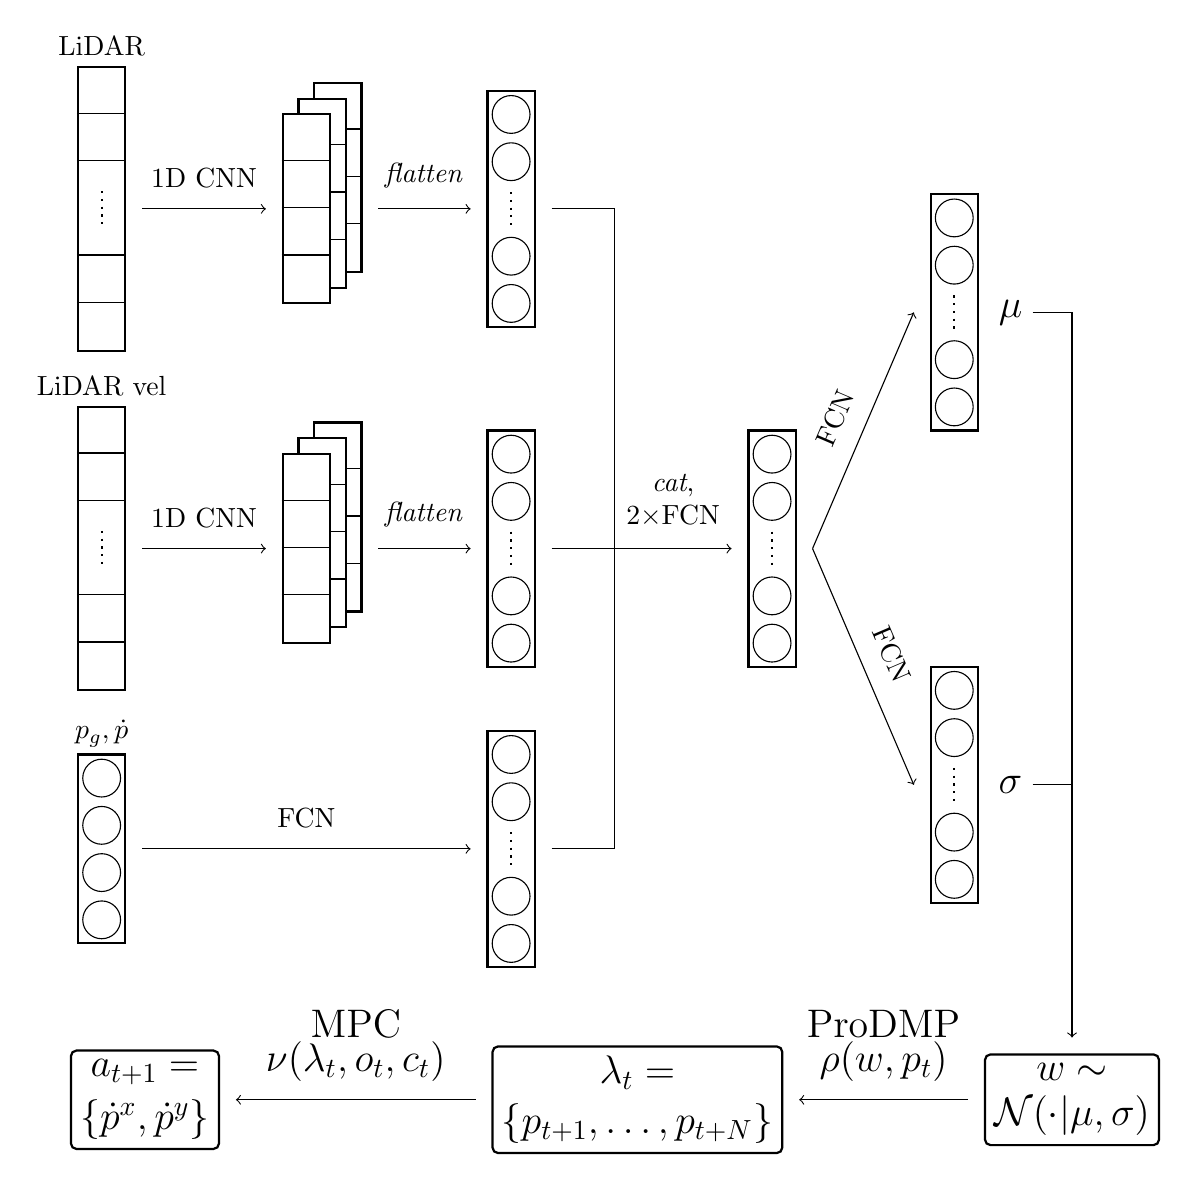
\begin{tikzpicture}[every node/.append style={align=center, thick}]
    \def\gridSize{6} % Number of squares per row and column
    \def\gridSizeIter{5} % Number of squares iteration, one less bc \gridSize - 1 not working in foreach
    \def\gridSizeCnn{4}
    \def\gridSizeCnnIter{3}
    \def\squareSize{0.6cm} % Size of each square

    % LiDAR obs
    \node[draw, minimum width=\squareSize, minimum height=\gridSize*\squareSize] (lidar) at (0, 0) {};
    \node (lidar_str) at ([yshift=2.5mm]lidar.north) {LiDAR};
    \foreach \i in {1,...,\gridSizeIter} {
      \ifnum \i = 3
            \draw[thick, dotted] ([yshift=-\i*\squareSize + 0.21cm]lidar.north) -- ([yshift=-\i*\squareSize - 0.21cm]lidar.north);
      \else
            \draw ([yshift=-\i*\squareSize]lidar.north west) -- ([yshift=-\i*\squareSize]lidar.north east);
       \fi
    }
    % LiDAR Vel obs
    \node[draw, minimum width=\squareSize, minimum height=\gridSize*\squareSize] (lidar_vel) at ([yshift=-2.5cm]lidar.south) {};
    \node (lidar_vel_str) at ([yshift=2.5mm]lidar_vel.north) {LiDAR vel};
    \foreach \i in {1,...,\gridSizeIter} {
      \ifnum \i = 3
            \draw[thick, dotted] ([yshift=-\i*\squareSize + 0.21cm]lidar_vel.north) -- ([yshift=-\i*\squareSize - 0.21cm]lidar_vel.north);
      \else
            \draw ([yshift=-\i*\squareSize]lidar_vel.north west) -- ([yshift=-\i*\squareSize]lidar_vel.north east);
       \fi
    }
    % Obs, goal position and velocity
    \node[draw, minimum width=\squareSize, minimum height=4*\squareSize] (obs) at ([yshift=-2cm]lidar_vel.south) {};
    \node (obs_str) at ([yshift=2.5mm]obs.north) {$\boldsymbol{p}_g, \dot{\boldsymbol{p}}$};
    \foreach \i in {0,...,3} {
       \draw ([yshift=-\i*\squareSize - \squareSize / 2 - 0.015cm]obs.north) circle (\squareSize / 2 - 0.06cm);
    }

    % LiDAR CNN
    \node[draw, fill=white, minimum width=\squareSize, minimum height=\gridSizeCnn*\squareSize] (cnn_lidar_2) at ([xshift=3cm,yshift=0.4cm]lidar) {};
        \foreach \i in {1,...,\gridSizeCnnIter} {
            \draw ([yshift=-\i*\squareSize]cnn_lidar_2.north west) -- ([yshift=-\i*\squareSize]cnn_lidar_2.north east);
        }

    \node[draw, fill=white, minimum width=\squareSize, minimum height=\gridSizeCnn*\squareSize] (cnn_lidar_1) at ([xshift=2.8cm,yshift=0.2cm]lidar) {};
        \foreach \i in {1,...,\gridSizeCnnIter} {
            \draw ([yshift=-\i*\squareSize]cnn_lidar_1.north west) -- ([yshift=-\i*\squareSize]cnn_lidar_1.north east);
        }
    \node[draw, fill=white, minimum width=\squareSize, minimum height=\gridSizeCnn*\squareSize] (cnn_lidar_0) at ([xshift=2.6cm]lidar) {};
        \foreach \i in {1,...,\gridSizeCnnIter} {
            \draw ([yshift=-\i*\squareSize]cnn_lidar_0.north west) -- ([yshift=-\i*\squareSize]cnn_lidar_0.north east);
        }
    \draw [->] ([xshift=0.2cm]lidar.east) -- ([xshift=-0.2cm]cnn_lidar_0.west)  node[midway, above, yshift=4pt] () {1D CNN};

    % LiDAR Vel CNN
    \node[draw, fill=white, minimum width=\squareSize, minimum height=\gridSizeCnn*\squareSize] (cnn_lidar_vel_2) at ([xshift=3cm,yshift=0.4cm]lidar_vel) {};
        \foreach \i in {1,...,\gridSizeCnnIter} {
            \draw ([yshift=-\i*\squareSize]cnn_lidar_vel_2.north west) -- ([yshift=-\i*\squareSize]cnn_lidar_vel_2.north east);
        }

    \node[draw, fill=white, minimum width=\squareSize, minimum height=\gridSizeCnn*\squareSize] (cnn_lidar_vel_1) at ([xshift=2.8cm,yshift=0.2cm]lidar_vel) {};
        \foreach \i in {1,...,\gridSizeCnnIter} {
            \draw ([yshift=-\i*\squareSize]cnn_lidar_vel_1.north west) -- ([yshift=-\i*\squareSize]cnn_lidar_vel_1.north east);
        }
    \node[draw, fill=white, minimum width=\squareSize, minimum height=\gridSizeCnn*\squareSize] (cnn_lidar_vel_0) at ([xshift=2.6cm]lidar_vel) {};
        \foreach \i in {1,...,\gridSizeCnnIter} {
            \draw ([yshift=-\i*\squareSize]cnn_lidar_vel_0.north west) -- ([yshift=-\i*\squareSize]cnn_lidar_vel_0.north east);
        }
    \draw [->] ([xshift=0.2cm]lidar_vel.east) -- ([xshift=-0.2cm]cnn_lidar_vel_0.west) node[midway, above, yshift=4pt] () {1D CNN};

    % MLP for obs
    \node[draw, minimum width=\squareSize, minimum height=5*\squareSize] (obs_mlp) at ([xshift=5.2cm]obs) {};
    \foreach \i in {0,...,4} {
        \ifnum \i = 2
            \draw[thick, dotted] ([yshift=-\i*\squareSize - \squareSize / 2  + 0.2cm]obs_mlp.north) -- ([yshift=-\i*\squareSize - \squareSize / 2  - 0.22cm]obs_mlp.north);
        \else
            \draw ([yshift=-\i*\squareSize - \squareSize / 2 - 0.015cm]obs_mlp.north) circle (\squareSize / 2 - 0.06cm);
        \fi
    }
    \draw [->] ([xshift=0.2cm]obs.east) -- ([xshift=-0.2cm]obs_mlp.west)  node[midway, above, yshift=4pt] () {FCN};

    % Flatten LiDAR
    \node[draw, minimum width=\squareSize, minimum height=5*\squareSize] (flat_lidar) at ([xshift=2.6cm]cnn_lidar_0) {};
    \foreach \i in {0,...,4} {
        \ifnum \i = 2
            \draw[thick, dotted] ([yshift=-\i*\squareSize - \squareSize / 2 + 0.2cm]flat_lidar.north) -- ([yshift=-\i*\squareSize - \squareSize / 2  - 0.22cm]flat_lidar.north);
        \else
            \draw ([yshift=-\i*\squareSize - \squareSize / 2 - 0.015cm]flat_lidar.north) circle (\squareSize / 2 - 0.06cm);
        \fi
    }
    \draw [->] ([xshift=0.6cm]cnn_lidar_0.east) -- ([xshift=-0.2cm]flat_lidar.west)  node[midway, above, yshift=4pt] () {\textit{flatten}};
    % Flatten LiDAR Vel
    \node[draw, minimum width=\squareSize, minimum height=5*\squareSize] (flat_lidar_vel) at ([xshift=2.6cm]cnn_lidar_vel_0) {};
    \foreach \i in {0,...,4} {
        \ifnum \i = 2
            \draw[thick, dotted] ([yshift=-\i*\squareSize - \squareSize / 2  + 0.2cm]flat_lidar_vel.north) -- ([yshift=-\i*\squareSize - \squareSize / 2  - 0.22cm]flat_lidar_vel.north);
        \else
            \draw ([yshift=-\i*\squareSize - \squareSize / 2 - 0.015cm]flat_lidar_vel.north) circle (\squareSize / 2 - 0.06cm);
        \fi
    }
    \draw [->] ([xshift=0.6cm]cnn_lidar_vel_0.east) -- ([xshift=-0.2cm]flat_lidar_vel.west)  node[midway, above, yshift=4pt] () {\textit{flatten}};

    \draw ([xshift=0.2cm]flat_lidar_vel.east) -- ([xshift=1cm]flat_lidar_vel.east);
    \draw ([xshift=0.2cm]flat_lidar.east) -| ([xshift=1cm]flat_lidar_vel.east);
    \draw ([xshift=0.2cm]obs_mlp.east) -| ([xshift=1cm]flat_lidar_vel.east);

    % FCN after cat
    \node[draw, minimum width=\squareSize, minimum height=5*\squareSize] (mlp_cat_0) at ([xshift=3cm]flat_lidar_vel.east) {};
    \foreach \i in {0,...,4} {
        \ifnum \i = 2
            \draw[thick, dotted] ([yshift=-\i*\squareSize - \squareSize / 2 + 0.2cm]mlp_cat_0.north) -- ([yshift=-\i*\squareSize - \squareSize / 2  - 0.22cm]mlp_cat_0.north);
        \else
            \draw ([yshift=-\i*\squareSize - \squareSize / 2 - 0.015cm]mlp_cat_0.north) circle (\squareSize / 2 - 0.06cm);
        \fi
    }
    \draw [->] ([xshift=1cm]flat_lidar_vel.east) -- ([xshift=-0.2cm]mlp_cat_0.west) node[midway, above, yshift=4pt] () {\textit{cat},\\ 2$\times$FCN};
    % Second FCN after cat
    %\node[draw, minimum width=\squareSize, minimum height=5*\squareSize] (mlp_cat_1) at ([xshift=2cm]mlp_cat_0.east) {$\vdots$};
    %\foreach \i in {0,...,4} {
    %    \ifnum \i = 2
    %    \else
    %        \draw ([yshift=-\i*\squareSize - \squareSize / 2 - 0.015cm]mlp_cat_1.north) circle (\squareSize / 2 - 0.06cm);
    %    \fi
    %}
    %\draw [->] ([xshift=0.2cm]mlp_cat_0.east) -- ([xshift=-0.2cm]mlp_cat_1.west)  node[midway, above, yshift=4pt] () {FCN};

    % Mean
    \node[draw, minimum width=\squareSize, minimum height=5*\squareSize] (mlp_mean) at ([yshift=-3cm, xshift=2cm]mlp_cat_0.east) {};
    \node (mlp_mean_str) at ([xshift=0.4cm]mlp_mean.east) {\Large $\sigma$};
    \foreach \i in {0,...,4} {
        \ifnum \i = 2
            \draw[thick, dotted] ([yshift=-\i*\squareSize - \squareSize / 2 + 0.2cm]mlp_mean.north) -- ([yshift=-\i*\squareSize - \squareSize / 2  - 0.22cm]mlp_mean.north);
        \else
            \draw ([yshift=-\i*\squareSize - \squareSize / 2 - 0.015cm]mlp_mean.north) circle (\squareSize / 2 - 0.06cm);
        \fi
    }
    \draw [->] ([xshift=0.2cm]mlp_cat_0.east) -- ([xshift=-0.2cm]mlp_mean.west)  node[midway, above, yshift=4pt, sloped] () {FCN};
    % STD
    \node[draw, minimum width=\squareSize, minimum height=5*\squareSize] (mlp_std) at ([yshift=3cm, xshift=2cm]mlp_cat_0.east) {};
    \node (mlp_std_str) at ([xshift=0.4cm]mlp_std.east) {\Large $\mu$};
    \foreach \i in {0,...,4} {
        \ifnum \i = 2
            \draw[thick, dotted] ([yshift=-\i*\squareSize - \squareSize / 2 + 0.2cm]mlp_std.north) -- ([yshift=-\i*\squareSize - \squareSize / 2  - 0.22cm]mlp_std.north);
        \else
            \draw ([yshift=-\i*\squareSize - \squareSize / 2 - 0.015cm]mlp_std.north) circle (\squareSize / 2 - 0.06cm);
        \fi
    }
    \draw [->] ([xshift=0.2cm]mlp_cat_0.east) -- ([xshift=-0.2cm]mlp_std.west)  node[midway, above, yshift=4pt, sloped] () {FCN};

    % Weight sampling
    \draw (mlp_std_str) -| ([xshift=0.5cm]mlp_mean_str.east);
    \draw (mlp_mean_str) -- ([xshift=0.5cm]mlp_mean_str.east);
    \node[rectangle, draw=black, rounded corners=2pt] (weights) at ([xshift=0.5cm, yshift=-4cm]mlp_mean_str.east) {\Large$\boldsymbol{w}\sim$ \\[1ex] \Large$\mathcal{N}(\cdot\vert\mu,\sigma)$};
    \draw [->] ([xshift=0.5cm]mlp_mean_str.east) -- ([yshift=0.2cm]weights.north);
    \node[rectangle, draw=black, rounded corners=2pt] (traj) at ([xshift=-4.4cm]weights.west) {\Large$\boldsymbol{\lambda}_t=$\\[1ex] \Large$\{\boldsymbol{p}_{t+1},\dots,\boldsymbol{p}_{t+N}\}$};
    \draw [->] ([xshift=-0.2cm]weights.west) -- ([xshift=0.2cm]traj.east) node[midway, above, yshift=3pt] () {\Large ProDMP \\ \Large $\rho(\boldsymbol{w}, \boldsymbol{p}_t)$};
    \node[rectangle, draw=black, rounded corners=2pt] (action) at ([xshift=-4.4cm]traj.west) {\Large$\boldsymbol{a}_{t+1}=$\\[1ex] \Large$\{\dot{p}^x,\dot{p}^y\}$};
    \draw [->] ([xshift=-0.2cm]traj.west) -- ([xshift=0.2cm]action.east) node[midway, above, yshift=3pt] () {\Large MPC \\ \Large $\nu(\boldsymbol{\lambda}_t,\boldsymbol{o}_t,\boldsymbol{c}_t)$};

\end{tikzpicture}
